\begin{frame}[plain]
    \begin{center}
        \vspace{48pt}
        {\huge\bf センサーを使った応用}
    \end{center}
\end{frame}

\begin{frame}
    \frametitle{センサーをピンにつけてみよう}
    \begin{center}
        \begin{columns}
            \begin{column}{0.48\textwidth}
                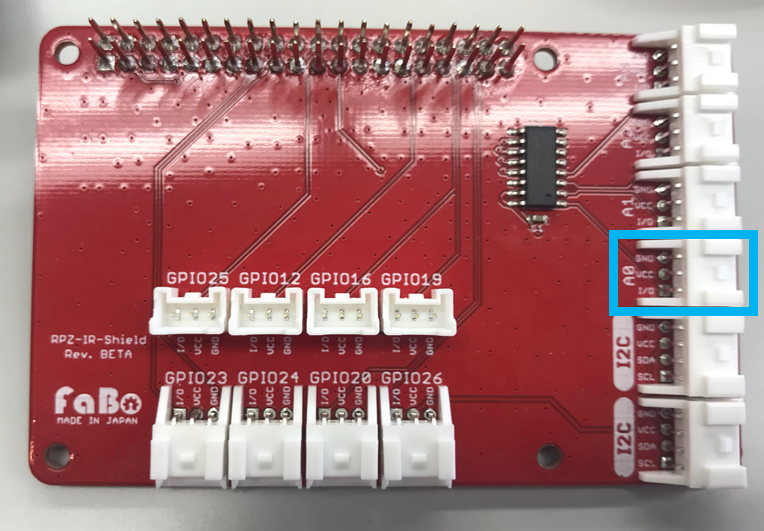
\includegraphics[width=0.8\textwidth]{images/chap05/text05-img030.png}
            \end{column}
            \begin{column}{0.48\textwidth}
                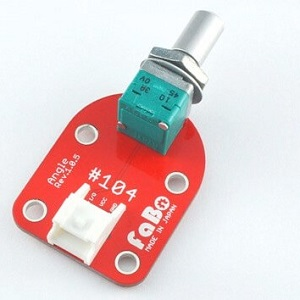
\includegraphics[width=0.8\textwidth]{images/chap05/text05-img022.jpg} 
            \end{column}
        \end{columns}
        \begin{itemize}
            \item A0とボリュームをつなげてみよう
            \item HSPで\textasciitilde/05/angle.hspを動かしてみよう
        \end{itemize}
    \end{center}
    \textpageref{22}
\end{frame}

\begin{frame}[fragile]
    \frametitle{ボリュームで画像を動かそう}
    \begin{lstlisting}[title=\textasciitilde/05/angle.hsp]
    #include "hsp3dish.as"
    #include "rpz-gpio.as"
    celload("hyou.png"),2
    p = 50
    spiopen 0

    *main
	    data = spiget(0,0)
	    p = rasp_map(data, 0, 1023, 0, 440)

	    redraw 0
	    pos 100,100
	    mes data
	    mes p
	    pos 0,0
	    celput 2
	    redraw 1

    	wait 10	
	    goto *main
    spiclose 0
    \end{lstlisting}
    \textpageref{22}
\end{frame}

\begin{frame}[fragile]
    \frametitle{入力の値の範囲を変える関数}
    \begin{center}
        \begin{figure}
            \includesvg[width=0.6\textwidth]{images/slide/rasp_map.svg}
        \end{figure}
        {rasp\_map(値,入力された値の最小サイズ,入力された値の最大サイズ,出力する値の最小サイズ,出力する値の最大サイズ)}
    \end{center}
    \textpageref{22}
\end{frame}

\begin{frame}[fragile]
    \frametitle{画像の場所}
    \begin{center}
        \begin{figure}
            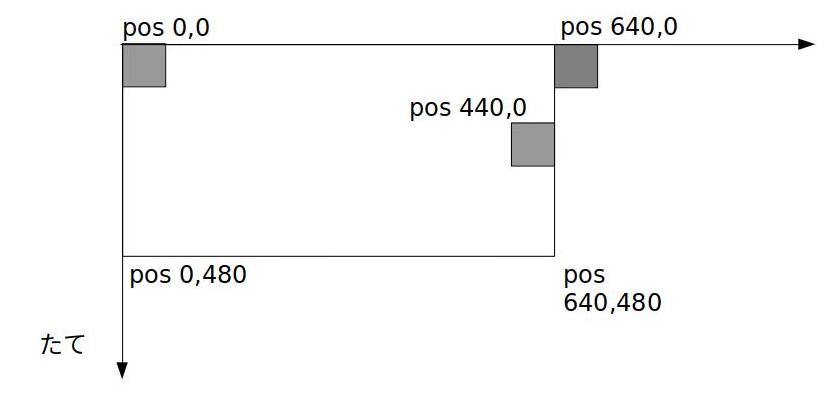
\includegraphics[width=\textwidth]{images/slide/volume_position.jpg}
        \end{figure}
        {画面のサイズは横が640、たてが480。\\
        今回の画像のサイズは横が200、たてが150。\\
        なので一番右に画像を置きたいときは、\\
        $\mbox{画面のサイズ}-\mbox{画像のサイズを考えよう}$}
    \end{center}
    \textpageref{22}
\end{frame}

\begin{frame}[fragile]
    \begin{exampleblock}{問題を解いてみよう}
    \begin{itemize}
        \item 教科書23ページ 問題5-10
        \begin{itemize}
            \item 6問は授業中にやる
        \end{itemize}
        \item 教科書24ページ 問題5-11
        \begin{itemize}
            \item 2問は宿題。時間があれば授業中にやる
        \end{itemize}
    \end{itemize}
    \end{exampleblock}
\end{frame}

\begin{frame}[fragile]
    \frametitle{LEDの明るさを変えよう}
    \begin{lstlisting}[title=\textasciitilde/05/pwm.hsp]
    #include "hsp3dish.as"
    #include "rpz-gpio.as"

    redraw 0
    redraw 1

    repeat
    gpio 27,1

    repeat 200
    if cnt < 10 : gpio 17,1 : else : gpio 17,0
    if cnt < 50 : gpio 18,1 : else : gpio 18,0
    if cnt < 100 : gpio 22,1 : else : gpio 22,0
    loop

    await 1
    loop

    gpio 17,0
    gpio 18,0
    gpio 22,0
    gpio 27,0
    stop
    \end{lstlisting}
    \textpageref{24}
\end{frame}

\begin{frame}
    \frametitle{LEDの明るさに強弱をつける}
    \begin{center}
        \begin{figure}
            \includesvg[width=0.8\linewidth]{images/chap05/led_frequency.svg}
        \end{figure}
        \begin{itemize}
            \item 一定時間のLEDの消灯時間の比率で明るさに強弱をつけることができる
        \end{itemize}
    \end{center}
    \textpageref{25}
\end{frame}